\documentclass[../main.tex]{subfiles}

\begin{document}

%%%%%%%%%%%%%%%%
% Intorduction to the coding interviews! %
%%%%%%%%%%%%%%%%
% \begin{chapquote}{Author's name, \textit{Source of this quote}}
% ``This is a quote and I don't know who said this.''
% \end{chapquote}
In  my humble opinion, I think it is a waste of our precious time to read either books or long blogs that purely focusing on the interview process and preparation. Personally, I would rather read a book that amuses me or work on my personal project that has some meanings or just enjoy it with your friends and families. 

% or in order to: know how each company hires their candidates and how to targeting each company by looking up
% This chapter is organized as: first, we introduce coding interviews taken by the tech companies in Section~\ref{section_coding_interview}. Next, in Section~\ref{section_leetcode}, we introduce LeetCode website~\footnote{https://leetcode.com/} and its problems. And how we can use this resource to help us with the coding interviews. Also, we provide other resources that can help you smooth your interview experience: including XX, iterviewing.io~\footnote{https://interviewing.io/}. 
This chapter consists of parts:
\begin{enumerate}
    \item Tech Interviews (Section.~\ref{section_coding_interview})
    \item Tips and Resources on Coding Interviews (Section.~\ref{}).
\end{enumerate}
%%%%%%%%%%%%%%%%
% section: Coding Interviews! %
%%%%%%%%%%%%%%%%
\section{Tech Interviews}
\label{section_coding_interview}
In this section, a brief introduction to the coding interviews and hiring process for a general software engineering position is first provided. , coding interviews related with data structures and algorithms are necessary. Your masterness of such knowledge varies as the requirement of more specific work. 

\subsection{Coding Interviews and Hiring Process}
Coding interviews, a.k.a whiteboard coding interviews, is one part of the whole interview process, where interviewees would be asked to solve one or a few well-defined problems and write down the code in 45-60 minutes of time window while the interviewer is watching. This process can be done either remotely via a shared file between interviewer and interviewee or face-to-face in a conference room on the whiteboard with the interviewer being present. 

Typically, the interview pipeline of software developer jobs consists of three stages--\textit{Exploratory chat with recruiter}, \textit{Screening interviews}, and \textit{On-site interviews}:
\begin{itemize}
    \item Exploratory chat with recruiters: Either you applied for the position and passed the initial screening or luckily get found by recruiters, they would contact you to schedule a short chat, normally through phone. During the phone call, the recruiter would introduce the company, the position, and ask for your field of interest; just to check the degree of interest on either side and decide if the process should be continued 
    \item Screening interviews: The screening interviews are usually two back-to-back coding interviews, each lasts 45-60 minutes. This process consists of the introduction on each side--interviewer and interviewee--which is cut as short as possible to save enough time for the coding interviews. 
    \item On-site interviews: If you have passed the first two rounds of interviews, you would be invited to the on-site interviews which is the most fun, exciting, but might also be the most daunting and tiring part of the whole process, since they can last anywhere from four hours to the entire day. The company would offer both transportation and accommodation to get you there. The on-site interview consists of 4 to 6 rounds one-on-one, each with an engineer in the team and lasts between 45-60 minutes; due to the long process, typically a lunch interview is included. There are some extra cases, which may or may not be included: group presentation, recruiter conversation, or conversation with the hiring manager or team manager. Presentation might happens to research scientist or higher-level positions. The onsite interview appears to be more more diverse compared with screening interview; introduction, coding interviews, brain teaser type of questions, behavior questions, and questions related to the field of the position, such as machine learning or web development. During the lunch interview, it was just hanging out with the one who is arranged to be with you, chatting while eating and showing you around the company in some cases. 
\end{itemize}
In some cases, you get to have to do on-line assignment which happens more to some start-ups and second tier tech companies, which requires you spending at least two hours solving problems without any promise that would lead to real interviews. Personally, I have done that twice with companies such as ; and I never heard back from them then. I fully resent such assignment; it is unfair because it wasted my time but not the company's, I learned nothing and the process is bored to hell! Ever since then I decide to stop the interview whenever such chore is demanded! 

Both the first and the second process serves as an initial screening process, the purpose is obviously; a trade-off because of the cost, because the remaining interview process can be quite costly in terms of finance--accommodation and transportation if you get  the on-site interviews--and in terms of time--the time cost on each side but mainly the cost from spending 5-8 hours on the interviewees from multiple engineers of the hiring company. 

Sometimes the process differs slightly between internship and full-time position; interns typically do not need on-site interviews. For new graduates, getting an internship first and through the internship to get a full-time offer can ease the whole job hunting process a bit. For more experienced engineers, they might get invited to on-site without the screening. 

\subsection{Why Coding Interviews?}
\subsubsection{The History} Coding interviews originated in the form of in-person interview and writing code on paper back in 1970s, populated as whiteboard interview in 1990s with the rise of the Internet, and froze in time and continued to live till today, 2020s.

Back in the 70s, computer time was expensive; the electricity, data processing and disc space costs were outrageous. Here shows the cost per megahertz from 1970 to 2007, courtesy off  Dr. Mark J. Perry:
\begin{figure}[h]
    \centering
    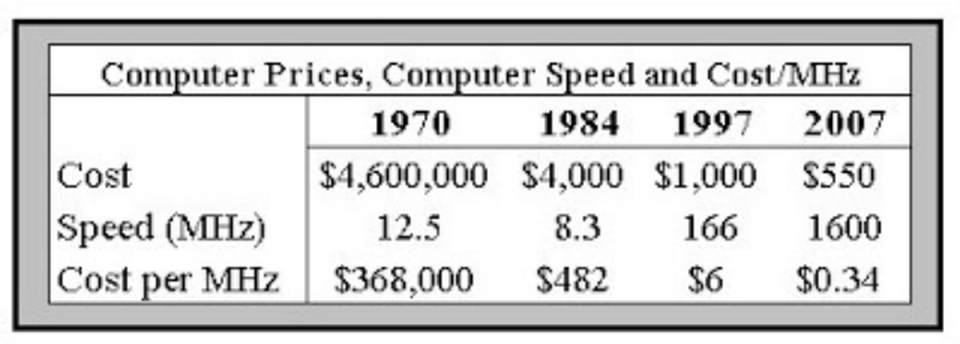
\includegraphics[width=0.8\columnwidth]{fig/mhz_640.jpg}
    \caption{Computer Prices, Computer Speed and Cost/MHz}
    \label{fig:interview_cost}
\end{figure}

Writing code on paper was a common, natural and effective way for programmers to code into computer later in this era. As Bill Gates describes the experience in a commencement speech at his alma mater -- Lakeside School: \textit{``You had to type up your program off-line and create this paper tape—and then you would dial up the computer and get on, and get the paper in there, and while you were programming, everybody would crowd around, shouting:``Hey, you made a typing mistake''``Hey, you messed this up''``Hey, you’re taking too much time.''}

Writing code is conducted on whiteboard rather than on paper in 1990s, when software engineering was growing exponentially with the rise of the Internet. It was a natural transition because the whiteboard is easy to setup, erase the mistake and the entire team can see the code which makes it a perfect way to conduct discussion. 

Now, at the 21st centry, when the computation is virtually free, the act of writing out the code on whiteboard or paper continues and part of our  interview process.

\subsubsection{Discussion}
Is it a good way to testify and select talented candidates? There are different opinions, in all, either favors it or oppose it. Stating the reason on each side is boring and not bear much value. Let us see what people say about it in their words.
\begin{drama}
\Character{Me}{me}
  \Character{Susie Chen}{susie}
  \Character{Eric Lin}{eric}
\mespeaks: How do you think about coding interviews?

\susiespeaks:  Ummmmmm well there was like one full month I only did Leetcode before interviewing with Facebok. LOL, was a bad experience but worth it hahahah. Susie was an intern from Facebook, with bachelor degree from University of.

\dotfill

\mespeaks: How the coding interview plays its role for new graduates and experienced engineers ?
\ericspeaks: 
\begin{itemize}
    \item Common: 
Both require previous proj demo/desc. Your work matters more than your score. Ppl care more about the actual experience than the paper work.\\
\item Diffs:
Grads are more asked for a passion or altitude of learning and problem-solving. For experienced engineers, the coding interview doesn't matter at all.
\end{itemize}
Eric is an Cloud Engineer at Contino, Four years of experience,  Master's degree in Information Technology at Monash University, Australia.
\end{drama}
%%%%%%%%%%%%%%%%
% Tips and Resources %
%%%%%%%%%%%%%%%%
\section{Tips and Resources}
Because of the focus of the book--learning computer science while having fun and the opinion I hold to coding interviews decide I will check this section short and offer more general information and tips. 
\subsection{Tips}
\paragraph{Tips for Preparation}
\begin{enumerate}
    \item First and of the most important tip: Do not be afraid of applying! Apply any company that you want to join and try your best to make it in the interviews. No need to check out statistics about their hiring ratio and be terrified of trying. You have nothing to lose and it would be a good chance to get first-hand interview experience with them, which might help you next time. So, be bold, and just do it! 
    \item Schedule your interviews with companies in a descending order of your favoritism. This way you get as much practice as possible before you go on with your dream company.
    \item Before doing real interviews, do mocking interviews; either ask your friends for help or find online mocking websites.
    \item If you are not fluent in English, practice even more using English! This is the situation for a lot of international STEM students, including me.
\end{enumerate}
I wished I would know the last three tips when I first started to prepare interview with Google back to 2016 (At least I followed the first tip, went for my dream company without hesitation, huh), one year in my PhD. It was a very first try, I prepared for a month(I mean at least 8 hours a day); reading and finishing all problems from \textit{Cracking the Coding Interview}. I failed the screening interview that is conducted through the phone with a Google share document. I was super duper nervous; taking long to just understand the question itself given my poor speaking English that time and the noise from the phone made the situation worse (talking with people on the phone fears me more than the ghost did from \textit{The Shining}, by Stephen King). At that time, I also did not have a clue about LeetCode. 

\paragraph{5 Tips for the Interview}
Here, we summarize five tips when we are doing a real interview or trying to mock one beforehand in the preparation. 
\begin{enumerate}
\item{Identify Problem Types Quickly:}
When given a problem, we read through the description to first understand the task clearly, and run small examples with the input to output, and see how it works intuitively in our mind. After this process, we should be able to identify the type of the problems. There are 10 main categories and their distrbution on the LeetCode which also shows the frequency of each type in real coding interviews. 
\begin{table}[h]
\label{tab: 1o_categories}
\centering
\noindent\captionof{table}{ 10 Main Categories of Problems on LeetCode, total 877 }
\resizebox{\columnwidth}{!}{\begin{tabular}{|c|c|c|c|c|}
  \hline
 Types & Count & Ratio1 & Ratio 2 \\ \hline
\multirow{2}{*}{Ad Hoc}  & Array &\\
                         & String &\\
                         \hline
\multirow{2}{*}{Complete search} & Iterative Search  & $84$& $27.8\%$ & $15.5\%$\\
    & Recursive Search   & $43$ & $22.2\%$ & $13.6\%$ \\\hline
%Binary Search  & $58$ & $18.6\%$ & $10.4\%$ \\ \hline
Divide and Conquer & $15$ & $8\%$ & $4.4\%$\\ 
Dynamic Programming & $114$ & $6.9\%$ & $3.9\%$\\ 
%Backtracking  & $39$ & $6.3\%$ & $3.5\%$\\ 
Greedy & $38$\\ \hline\hline
Math and Computational Geometry  & $103$ & $3.88\%$ & $2.2\%$ \\
Bit Manipulation & $31$ & $2.9\%$ & $1.6\%$\\ \hline
Total & $490$ & $N/A$ & $55.8\%$\\ \hline
 \end{tabular}}
\end{table}

\item{Do Complexity Analysis:}
We brainstorm as many solutions as possible, and with the given maximum input size $n$ to get the upper bound of time complexity and the space complexity to see if we can get AC while not LTE. 

For example, For example, the maximum size of input n is 100K, or $10^5$ (1K = 1, 000), and your algorithm is of order $O(n^2)$. Your common sense told you that $(100K)^2$ is an extremely big number, it is
$10^10$. So, you will try to devise a faster (and correct) algorithm to solve the problem, say of order $O(n\log_2{n})$. Now $10^5\log_2{10^5}$ is just $1.7\times 10^6$. Since computer nowadays are quite fast and can
process up to order 1M, or $10^6$ (1M = 1, 000, 000) operations in seconds, your common sense told you that this one likely able to pass the time limit.

\item{ Master the Art of Testing Code:}
We need to design good, comprehensive, edges cases of test cases so that we can make sure our devised algorithm can solve the problem completely while not partially. 

\item {Master the Chosen Programming Language:}
\end{enumerate}
\subsection{Resources}
\label{section_resource}
\subsubsection{Online Judge System}
\paragraph{Leetcode} LeetCode is a website where you can practice on real interviewing questions used by tech companies such as Facebook, Amazon, Google, and so on. 

Here are a few tips to navigate the usage of LeetCode:
\begin{itemize}
\begin{figure}[!ht]
    \centering
    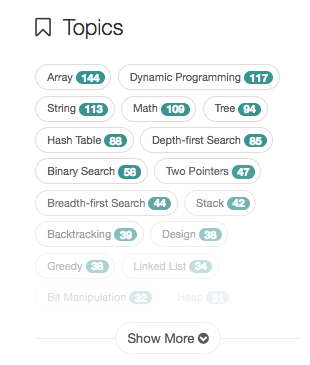
\includegraphics[width=0.6\columnwidth]{fig/category_tag.png}
    \caption{Topic tags on LeetCode}
    \label{fig:category_tag}
\end{figure}
    \item \textbf{Use category tag to focusing practice:} With the category or topic tags, it is better strategy to practice and solve problems one type after another, shown in Fig.~\ref{fig:category_tag}. 

\item \textbf{Use test case to debug:} Before we submit our code on the LeetCode, we should use the test case function shown in Fig.~\ref{fig:test_case} to debug and testify our code at first. This is also the right mindset and process at the real interview. 
\begin{figure}[h]
    \centering
    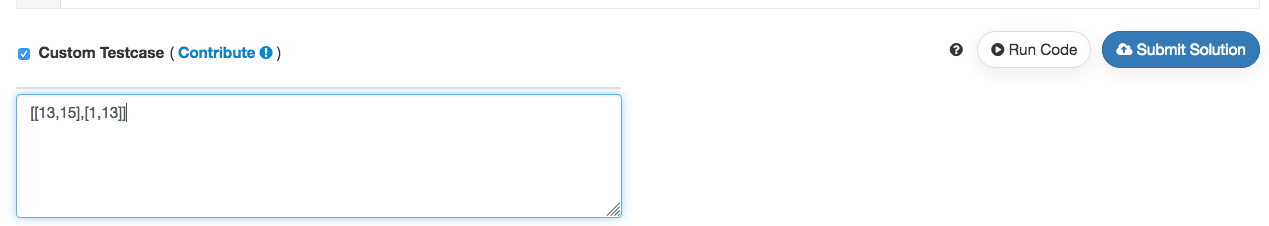
\includegraphics[width=0.8\columnwidth]{fig/test_case_leetcode.png}
    \caption{Use Test Case to debug}
    \label{fig:test_case}
\end{figure}

\item \textbf{Use Discussion to get more solutions:}
\begin{figure}[h]
    \centering
    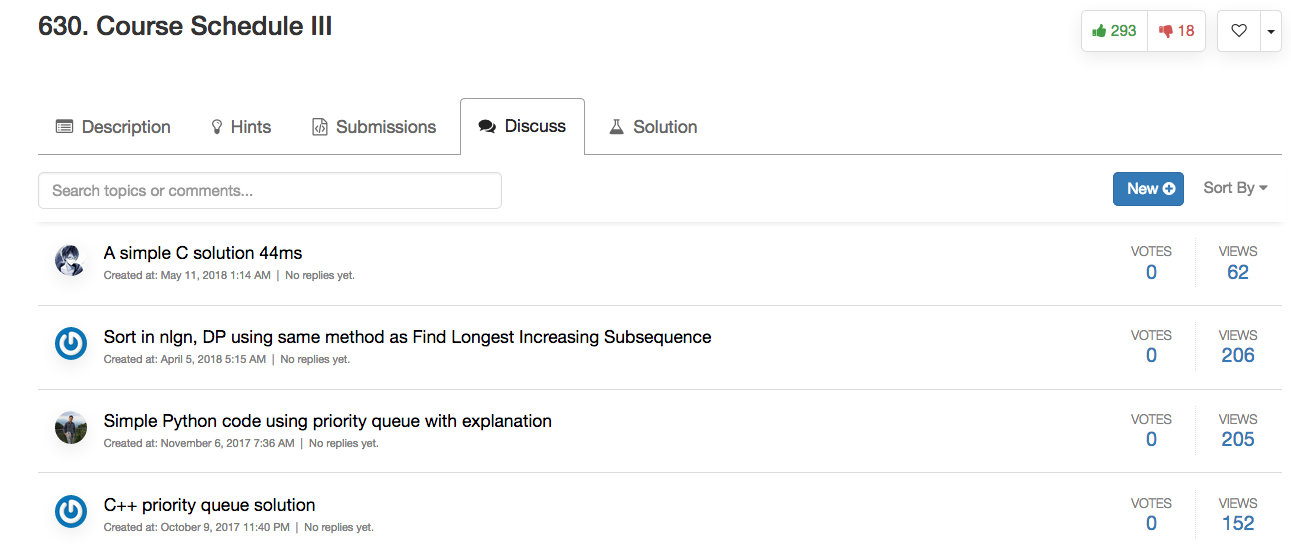
\includegraphics[width=0.8\columnwidth]{fig/leetcode_discussion.png}
    \caption{Use Test Case to debug}
    \label{fig:test_case}
\end{figure}
\begin{table}[!ht]
\begin{small}
\centering
\noindent\captionof{table}{ Problems categorized by data structure on LeetCode, total 877 }
 \noindent \begin{tabular}{|p{0.25\columnwidth}|p{0.25\columnwidth}| p{0.25\columnwidth}| p{0.25\columnwidth}|}
  \hline
 Data Structure & Count & Percentage/Total Problems & Percentage/Total Data Structure \\ \hline
Array  & $136$& $27.8\%$ & $15.5\%$\\
String   & $109$ & $22.2\%$ & $13.6\%$ \\ \hline

Linked List & $34$ & $6.9\%$ & $3.9\%$\\ 
Hash Table & $87$ \\ \hline

Stack & $39$ & $8\%$ & $4.4\%$\\ 
Queue & $8$ & $1.6\%$ & $0.9\%$\\ \hline 

Heap  & $31$ & $6.3\%$ & $3.5\%$\\
Graph & $19$ & $3.88\%$ & $2.2\%$ \\\hline

Tree  & $91$ & $18.6\%$ & $10.4\%$ \\ 
Binary Search Tree &$13$ \\
Trie & $14$ & $2.9\%$ & $1.6\%$\\
Segment Tree & $9$ & $1.8\%$ & $1\%$ \\\hline

Total & $490$ & $N/A$ & $55.8\%$\\ \hline
\end{tabular}
  \label{tab:msrc_precession}
  \end{small}
\end{table}

\begin{table}[h]
\label{tab: 1o_categories_2}
\centering
\noindent\captionof{table}{ 10 Main Categories of Problems on LeetCode, total 877 }
 \noindent \begin{tabular}{|p{0.28\columnwidth}|p{0.24\columnwidth}| p{0.24\columnwidth}| p{0.24\columnwidth}|}
  \hline
 Algorithms & Count & Percentage/Total Problems & Percentage/Total Data Structure \\ \hline
Depth-first Search  & $84$& $27.8\%$ & $15.5\%$\\
Breadth-first Search   & $43$ & $22.2\%$ & $13.6\%$ \\
Binary Search  & $58$ & $18.6\%$ & $10.4\%$ \\ \hline
Divide and Conquer & $15$ & $8\%$ & $4.4\%$\\ 
Dynamic Programming & $114$ & $6.9\%$ & $3.9\%$\\ 
Backtracking  & $39$ & $6.3\%$ & $3.5\%$\\ 
Greedy & $38$\\ \hline
Math & $103$ & $3.88\%$ & $2.2\%$ \\
Bit Manipulation & $31$ & $2.9\%$ & $1.6\%$\\ \hline
Total & $490$ & $N/A$ & $55.8\%$\\ \hline
  \end{tabular}
\end{table}
\end{itemize}
\paragraph{Algorithm Visualizer} If you are inspired more by visualization, then check out this website, \url{https://algorithm-visualizer.org/}. If offers us a tool to visualize the running process of algorithms.
\subsubsection{Mocking Interviews Online}
\paragraph{Interviewing.io} Use the website interviewing.io, you can have real mocking interviews given by software engineers working in top tech company. This can greatly help you overcome the fear, tension. Also, if you do well in the practice interviews, you can get real interviewing opportunities from their partnership companies. 

Interviewing is a skill that you can get better at. The steps mentioned above can be rehearsed over and over again until you have fully internalized them and following those steps become second nature to you. A good way to practice is to find a friend to partner with and the both of you can take turns to interview each other.

A great resource for practicing mock coding interviews would be interviewing.io. interviewing.io provides free, anonymous practice technical interviews with Google and Facebook engineers, which can lead to real jobs and internships. By virtue of being anonymous during the interview, the inclusive interview process is de-biased and low risk. At the end of the interview, both interviewer and interviewees can provide feedback to each other for the purpose of improvement. Doing well in your mock interviews will unlock the jobs page and allow candidates to book interviews (also anonymously) with top companies like Uber, Lyft, Quora, Asana and more. For those who are totally new to technical interviews, you can even view a demo interview on the site (requires sign in). Read more about them here.

Aline Lerner, the CEO and co-founder of interviewing.io and her team are passionate about revolutionizing the technical interview process and helping candidates to improve their skills at interviewing. She has also published a number of technical interview-related articles on the interviewing.io blog. interviewing.io is still in beta now but I recommend signing up as early as possible to increase the likelihood of getting an invite.

\paragraph{Pramp} Another platform that allows you to practice coding interviews is Pramp. Where interviewing.io matches potential job seekers with seasoned technical interviewers, Pramp takes a different approach. Pramp pairs you up with another peer who is also a job seeker and both of you take turns to assume the role of interviewer and interviewee. Pramp also prepares questions for you, along with suggested solutions and prompts to guide the interviewee.

\subsubsection{Communities}
If you understand Chinese, there is a good community~\footnote{http://www.1point3acres.com/bbs/} that we share information with either interviews, career advice and job packages comparison. 

\end{document}